\section{Simulation Results}%
\label{sec:simulations}

The simulation section illustrates the results in the order of detection, estimation and joint detection and estimation.
Four different lengths of reference symbol sequences are simulated with $50\%$ rolloff Square-Root Raised Cosine (SRRC) pulses.
The reference sample sequence is chosen from Gold sequence and modulated by a QPSK alphabet with good autocorrelation properties.
We assume the normalized frequency offset is small enough so that the design parameter $k$ of the SD estimator
can be chosen optimally by $2/3$ length of the preamble (For $K-$SD estimator, all the estimates of SD satisfying the aliasing limits). 
% may give more sentence here.

\subsection{Simulation Results for Detection}

\begin{figure}[t]
    \centerline{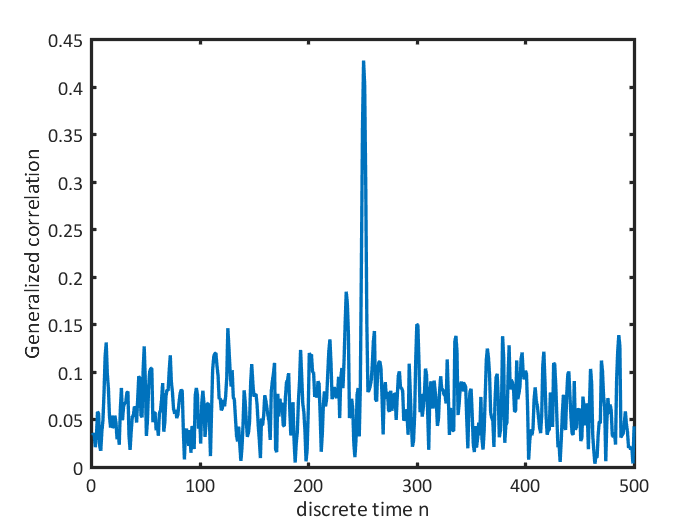
\includegraphics[width=3.4in]{generalized_correlation.png}}
    \caption{Performance of GLRT detector of~\eqref{eq:generalized_corr} at each delay of received stream (no fractional delay, dashed line: the position of $\bar{p}$)}
    \label{fig:Generalized correlation}
    \end{figure}

\begin{figure}[t]
    \centerline{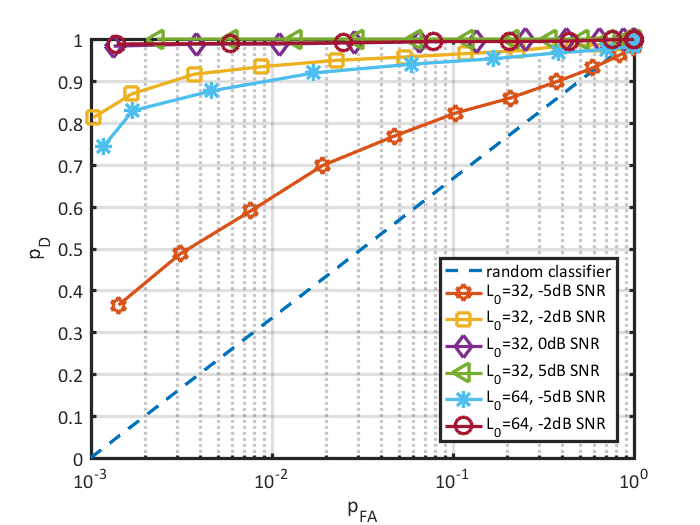
\includegraphics[width=3.4in]{receiver_operating_characteristics.png}}
    \caption{Receiver operating characteristics of GLRT based detector for different lengths of reference sequence and SNR}
    \label{fig:Receiver operating characteristics}
    \end{figure}

\begin{figure}[t]
    \centerline{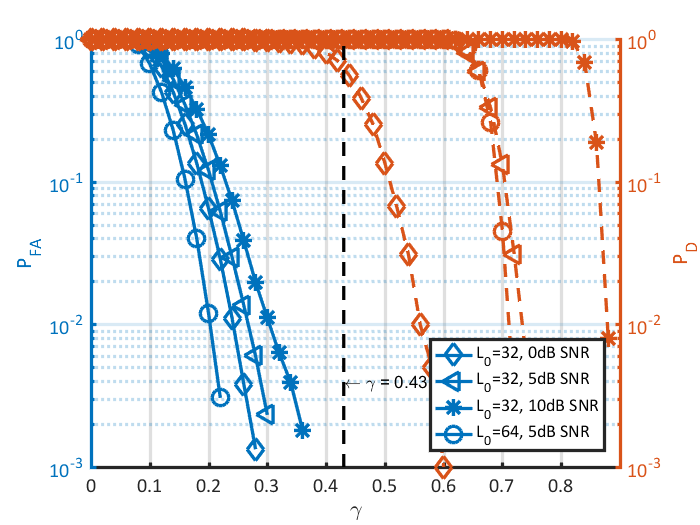
\includegraphics[width=3.4in]{false_alarm_and_detection_probability.png}}
    \caption{False alarm and detection ratio for different SNR and sizes of preamble ($M=4$. Blue: false alarm probability. Red: detection probability)}
    \label{fig:False alarm and detection}
    \end{figure}

\begin{figure}[t]
    \centerline{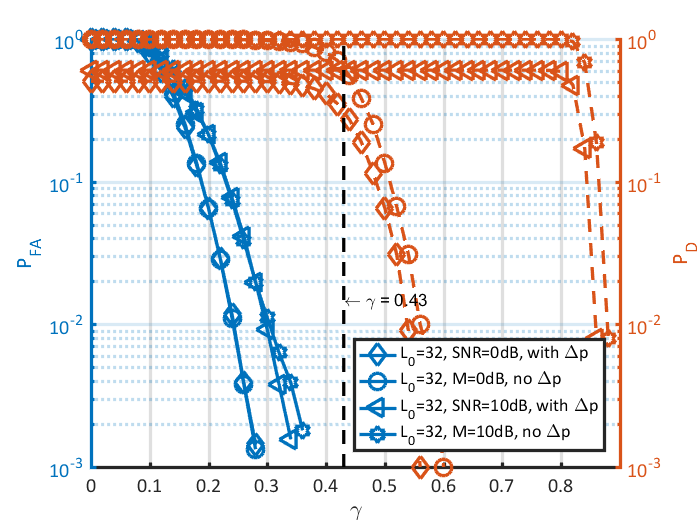
\includegraphics[width=3.4in]{false_alarm_and_detection_probability_fractional_delay.png}}
    \caption{Comparison between false alarm and detection ratio with and without maximum $\Delta p$ for same $L_0$ and different SNR ($M=4$. Blue: $P_{\text{FA}}$. Red: $P_{\text{D}}$)}
    \label{fig:False alarm and detection with frac delay}
    \end{figure}

In this section, we first illustrate the simulation results of the detection algorithm without considering the fractional delay.
The effect of fractional delay on detection will be discussed at the end of this section. 

Figure~\ref{fig:Generalized correlation} illustrates the performance of the proposed detector in~\eqref{eq:generalized_corr} without fractional delay for 
$L_0=32$, $M=8$,~\numb{0}\dB~SNR. The GLRT based detector performs robust at low SNR since it achieves the highest generalized correlation at $\bar{p}$.
However, from the adjacent correlations centered at $\bar{p}$ that we point out,
the correlation decays very slow and thus it will make much more challenging to choose the threshold to distinguish between 
the true position of received sequence and its corresponding adjacent positions. This is due to pulse shaping and oversampling. Specifically,
the width of "mainlobe" depends on the shape of pulse and the value of $M$, e.g., 
it will become wider if $M$ is larger. 
To accommodate this imperfect autocorrelation influence by pulse shaping and oversampling, we adjust the detection algorithm by finding the local maximum of the correlation near $\bar{p}$ instead of
just comparing the correlations with threshold to make the decisions at each delay. 

Figure~\ref{fig:Receiver operating characteristics} shows the receiver operating characteristics (ROC) of the proposed (adjusted) detector.
It basically illustrates that the detector has good ROCs at very low SNR. Specifically, the detector achieves perfect ROCs for positive SNR for all length of $L_0$; 
Moreover, it is still robust to negative SNR environment. For instants, we can select such a threshold to achieve  
$P_{\text{FA}} \approx 10^{-3}$ and $P_{\text{D}} \geq 0.8$ simultaneously when $L_0=32$ and SNR $=$~\numb{-2}\dB.
However, it is not clear from this figure to pick an exact threshold for certain detection purpose.

Figure~\ref{fig:False alarm and detection} shows the performance of detector but from another perspective. Specifically, it gives us a deep insight into
the false alarm and detection probabilities versus the threshold. 
Basically, we have two observations. First, compared with the two curves of~\numb{0}dB~and~\numb{10}dB SNR for $L_0=32$,
we see the latter needs to achieve the same false alarm probability with a higher threshold. This is because the level of "sidelobe" in Figure~\ref{fig:Generalized correlation} is
increasing in terms of SNR; If we look at the same two curves of $P_{\text{D}}$, the curve of a high SNR maintains a perfect $P_{\text{D}}$ at a higher threshold. This is due to
the increasing level of "mainlobe" via SNR. Second, compared with two curves with different $L_0$ and same SNR, we see that the received sequence with more symbols achieves the same $P_{\text{FA}}$
at lower threshold. The reason is that the sequence with more symbols will have a better autocorrelation property.  
Moreover, it is commonly hard to pick such a threshold to accommodate all specific detection purposes.
For simulation purpose, now if we want to determine a threshold to work for all reference sequences with $L_0 {\geq} 32$ and SNR up to~\numb{10}\dB,
based on Figure~\ref{fig:False alarm and detection} and Neyman-Pearson criterion, $\gamma=0.43$ is a good choice to meet $P_{\text{FA}}<1e^{-3}$ and nearly perfect $P_{\text{D}}$ for all lengths of $L_0$.

To this point, we discuss the effect of fractional delay $\Delta p$ in model~\eqref{eq:model} on modified detection algorithm. 
Above, we assume $\Delta p$ is neglected when sampling rate $f_s$ is sufficiently large. 
However, when $f_s$ is not much bigger than symbol rate, 
or equivalently, the oversampling factor $M$ is relatively small, 
the value of $\Delta p$ will degrade the performance of detection and estimation due to
mismatching between the preamble in received and reference sequence.
For example, when $M{=}1$ and the preamble has the maximum fractional delay 
equaling to $\Delta p=\pm\frac{1}{2f_s}=\pm\frac{T}{2M}=\pm\frac{T}{2}$, 
half of the preamble in received and reference sequence is mismatched thus the peak of
generalized correlation in Figure~\ref{fig:Generalized correlation} will disappear.
Instead, Two peaks will show up: one at $\bar{p}$ and another one at the adjacent $p$ depending on the sign of $\Delta p$.
Recall, the detection algorithm is to find the local maximum of generalized correlation around $\bar{p}$.
Thus, there is no doubt that $\Delta p$ will greatly decrease the detection probability, as shown in Figure~\ref{fig:False alarm and detection with frac delay}.

In Figure~\ref{fig:False alarm and detection with frac delay}, the most intuitive observation is that the curves of $P_{\text{D}}$ with (maximum) fractional delay for all SNR
do not start at 1 when $\gamma$ is very low. The detector is hard to make the correct decision between the adjacent two delays with similar high correlations. 
If we compare with the two curves of $P_{\text{D}}$ for SNR $=\numb{0}\dB$ and $\numb{10}\dB$
both with fractional delay, the initial $P_{\text{D}}$ of $\numb{10}\dB$ SNR is approxmiately 0.6 and greater than 0.5 at $\numb{0}\dB$.
This is because at low SNR, the noise level degrades the detection performance; While, at high SNR, 
the percentage of the mismatched preamble between received and reference sequence 
is below $50\%$ since $\Delta p{=}{\pm}\frac{T}{2M}{=}{\pm}\frac{T}{8}$. The generalized correlation
at $\bar{p}$ will be larger than at the adjacent delay with the probability more than $1/2$.

We can also see the fractional delay has a small effect on false alarm probability, which is important. For example, as we discussed above,
if we want to choose a threshold to work for the detection task that all reference sequences with $L_0 {\geq} 32$
and SNR${\leq}$\numb{10}\dB, then from Figure~\ref{fig:False alarm and detection} and~\ref{fig:False alarm and detection with frac delay},
$\gamma=0.43$ is still a good choice to meet the requirement of false alarm probability. Note, when $\Delta p$ is large, although $\Delta p$ will "lead" the 
detector to make the decision between the two adjacent delays with similar highest generalized correlation,
we can just keep either one as the detection result but care more about the estimation accuracy with the determined received sequence
for coherent demodulation. Thus, in the next section, we will talk about the degradation of estimation accuracy with different levels of $\Delta p$.
The goal is to choose the oversampling factor $M$ that makes the estimation error negligible.

\subsection{Simulation Results for Estimation}

\begin{figure}[t]
    \centerline{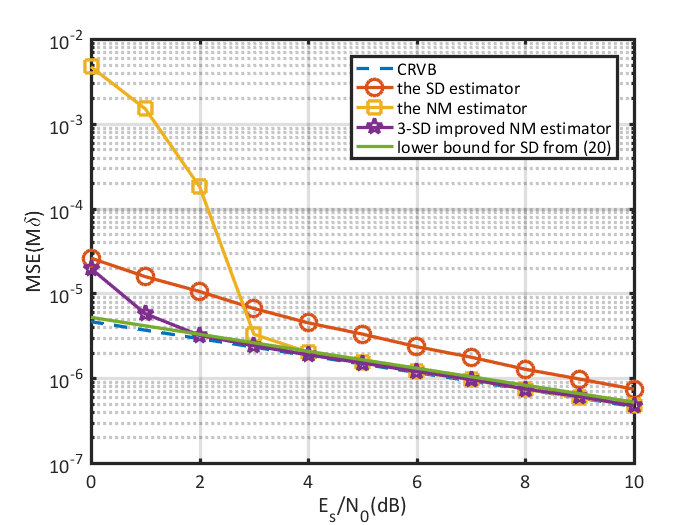
\includegraphics[width=3.4in]{accuracy_NM_SD.png}}
    \caption{Accuracy of the SD and SD (or $K$-SD) based NM estimators ($L_0=32$)}
    \label{fig:accuracy_NM_SD}
    \end{figure}

\begin{figure}[t]
    \centerline{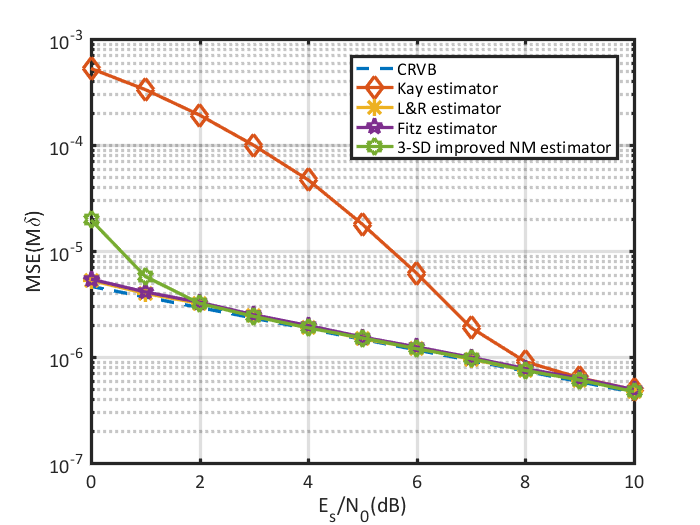
\includegraphics[width=3.4in]{accuracy_NM_traditional.png}}
    \caption{Accuracy of the NM estimator and conventional estimators ($L_0=32$)}
    \label{fig:accuracy_NM_traditional}
    \end{figure}

\begin{figure}[t]
    \centerline{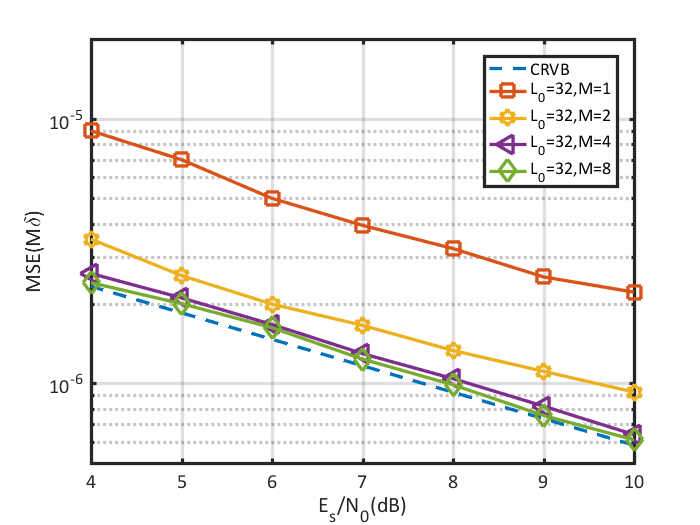
\includegraphics[width=3.4in]{accuracy_NM_with_M_frac.png}}
    \caption{Accuracy of NM estimator with maximum fraction delay for different value of oversampling factor ($L_0=32$, $\Delta p=\frac{T}{2M}$)}
    \label{fig:accuracy_NM_with_M_frac}
    \end{figure}

\begin{figure}[t]
    \centerline{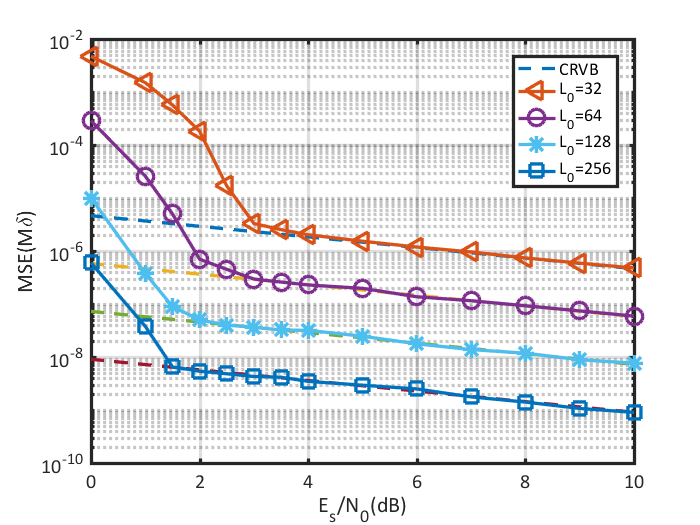
\includegraphics[width=3.4in]{freq_NM_with_different_size.png}}
    \caption{Accuracy of NM frequency estimate in joint detection and estimation ($\gamma=0.43$, $M=4$, $\Delta p \in (-\frac{T}{8},\frac{T}{8}]$)}
    \label{fig:accuracy_freq_NM_joint}
    \end{figure}

\begin{figure}[t]
    \centerline{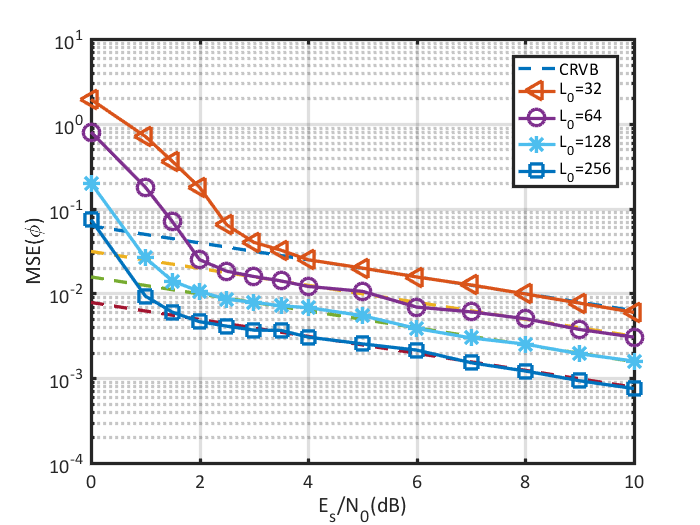
\includegraphics[width=3.4in]{phi_NM_with_different_size.png}}
    \caption{Accuracy of the NM phase estimate in joint detection and estimation ($\gamma=0.43$, $M=4$, $\Delta p \in (-\frac{T}{8},\frac{T}{8}]$)}
    \label{fig:accuracy_phi_NM_joint}
    \end{figure}

In this section, we focus on the estimating accuracy of our proposed estimators (SD, or $K-$SD and NM)
by assuming no fractional delay and the sequential GLRT detection progress is perfect.
The simulation shows the NM estimator can achieve as good accuracy as those conventional estimators in ~\cite{Kay_89,Luise_Reggiannini_95,Fitz_94}
for coherent demodulation at moderate SNR. 
Then, the effect of fractional delay $\Delta p$ on estimating accuracy with respect to $M$ will be discussed.
We find that $M=4$ yields a negligible estimation error from $\Delta p$.
At the end of this section, we will also show the estimating accuracy of NM estimator after joint detection and simulation for coherent demodulation.  

Figure~\ref{fig:accuracy_NM_SD} gives the insight into the accuracy of two proposed estimators.
The lower dashed line denotes the Cramer-Rao vec-tor bound (CRVB) for frequency estimate in~\eqref{eq:model}
multiplied by $M$, which is given by

\begin{equation}
    \label{eq:CRVB_freql}
    \text{CRVB}(M\delta) \geq \frac{3}{2\pi^{2}L_{0}^3E_s/N_{0}}.
  \end{equation}
Furthermore, the CRVB for $\phi$ is derived as

\begin{equation}
    \label{eq:CRVB_phi}
    \text{CRVB}(\phi) \geq \frac{2}{L_{0}E_s/N_{0}}.
  \end{equation}
The derivation steps of~\eqref{eq:CRVB_freql} and~\eqref{eq:CRVB_phi} are given in Appendix~\ref{BL}.
In Figure~\ref{fig:accuracy_NM_SD}, we see the NM estimator approaches the CRVB at SNR$=\numb{4}\dB$. 
Note, the accuracy of the SD estimator is crucial
not only just for building the GLRT detector but deciding the accuracy of the NM estimator.
The evidence is that the NM estimator performs even worse than the SD estimator at low SNR.
This is because the Newton iteration of~\eqref{eq:iter_NM_est} converges occasionally to local
minimum away from the true frequency offset if the initial (SD) estimate is far from the true frequency offset. 
Moreover, Figure~\ref{fig:accuracy_NM_SD} shows the averaging method of~\eqref{eq:K_SD_est}
improves the accuracy of the SD estimator thus improves the NM estimator at low SNR.

Figure~\ref{fig:accuracy_NM_traditional} compares the performance of the NM estimator and conventional estimators in ~\cite{Kay_89,Luise_Reggiannini_95,Fitz_94}.
Related to Figure~\ref{fig:accuracy_NM_SD}, we co-nclude that the NM estimator can achieve as good accuracy as those autocorrelation-based estimators 
(L\&R estimator~\cite{Luise_Reggiannini_95} and Fitz estimator~\cite{Fitz_94})
when the SD estimator is accurate enough. Put it another way, without increasing complexity by averaging with multiple SD estimators, 
the NM estimator can achieve the same good accuracy as the traditional estimators at moderate SNR.

Now we are going to discuss the effect of $\Delta p$ on estimating accuracy of the NM estimator.
In the previous section, we got the conclusion that $\Delta p$ both degrades the detection probability
and estimating accuracy because of the mismatching between the preamble in received and reference sequence.
The solution to dealing with the degradation of detection is to maintain the decision of detector but sacrifice the 
accuracy of the estimator. Thus, we need to select the oversampling factor $M$ that makes the fractional delay $\Delta p$ small enough and the estimation error negligible.  
Figure~\ref{fig:accuracy_NM_with_M_frac} illustrates the estimating accuracy of NM estimator with maximum fractional delay
equaling to $\Delta p{=}\frac{T}{2M}$ for different $M$. It can be seen that when $M=1,2$, i.e., $\Delta p=\frac{T}{2},\frac{T}{4}$, the gap between
the mean-squared error (MSE) and the CRVB is obvious; The MSE of two curves for $M=4$ and $M=8$ both nearly approach the
CRVB. But note, the reference sequence with $M=8$ induces an extra double computational complexity than $M=4$. Thus, $M=4$ is an ideal choice
for joint detection and estimation purpose in this paper.

At end of simulation section, the complete signal acquisition chain (joint detection and estimation) in Figure~\ref{fig:sig_acquis_chain} is simulated.
Figure~\ref{fig:accuracy_freq_NM_joint} and~\ref{fig:accuracy_phi_NM_joint} illustrate the performance of NM estimator after joint detection and 
estimation. $\Delta p$ is included with the range determined by $M$.
The parameters, e.g., the value of $\gamma$, the oversampling factor $M$, are chosen based on the previous discussion.
No averaged SD estimator is used because we want to reduce the complexity of the sequential detection process.
Compared with Figure~\ref{fig:False alarm and detection} and Figure~\ref{fig:accuracy_NM_SD}, the reason for the NM estimator not approaching the CRVB at low SNR
is due to non-sufficient accuracy of the SD estimator. Besides that, we can get a common conclusion that by increasing
the size of the preamble, better performance of carrier synchronization is realized and CRVB is approached at lower SNR.


